\chapter{MARCO METODOLÓGICO}

El trabajo de investigación se divide en los siguientes tres frentes: nodo sensor, aplicación web y gateway. En este sentido, se ha optado por dividir la metodología para tener una mejor documentación del proceso a seguir en cada frente del proyecto, tanto en la selección de los componentes electrónicos empleados y los protocolos de comunicación inalámbrica más eficientes, así como de las tecnologías empleadas para la selección.

\begin{itemize}
    \item \textbf{Desarrollo de nodo sensor}
    \item \textbf{Desarrollo de la aplicación web}
    \item \textbf{Configuración del gateway}
    \item \textbf{Desarrollo del subsistema de mitigación activa y control}
\end{itemize}

\section{Metodologías de investigación}

\subsection{Metodología V model}
Para el desarrollo de la aplicación web, se ha escogido la metodología V model. Esta metodología permite estructurar y gestionar de manera eficaz el proceso de desarrollo y prueba, asegurando que cada fase de construcción esté alineada con un proceso de validación correspondiente. A continuación se describe la adaptación de este modelo al desarrollo de la aplicación web de monitoreo de datos de CO\(_2\).

\begin{figure}[H]
    \centering
    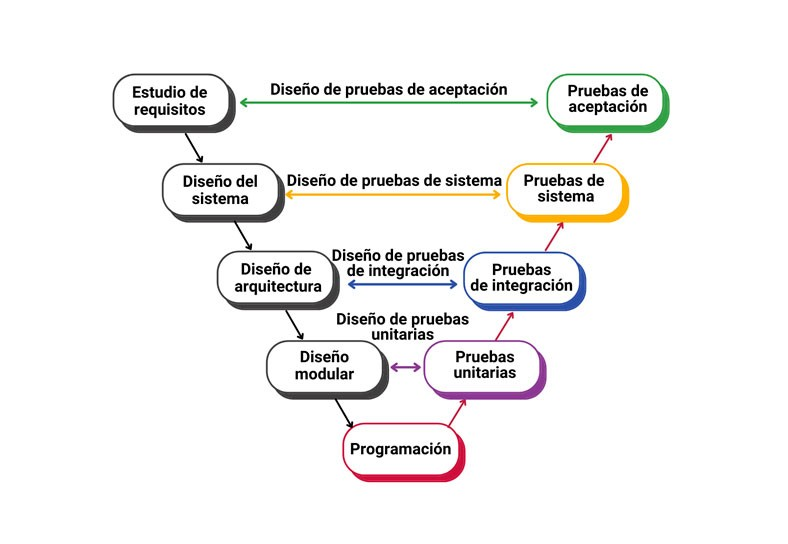
\includegraphics[width=0.9\linewidth]{images/capitulo3/vmodel.png}
    \caption{\centering Metodología V model \cite{vmodel}.}
    \label{fig:vmodel}
\end{figure}



\subsubsection{Definición de Requisitos}

En esta primera etapa, se establecen los requisitos funcionales y no funcionales de la aplicación web. Estos incluyen la capacidad para recibir y mostrar los datos provenientes del mega gateway Kona, almacenar y consultar dichos datos en una base de datos SQL, y activar alertas visuales y sonoras cuando los niveles de CO\(_2\) superen un umbral predeterminado.

\subsubsection{Diseño de Sistema y Arquitectura}

En esta fase, se desarrolla una arquitectura que permita la integración de todos los componentes necesarios para la recepción, almacenamiento y visualización de los datos. Se emplea la arquitectura por capas, la cual a su vez considera el uso de un backend basado en C\# y .NET, una API para la comunicación entre el backend y el frontend, y un frontend en React, con TypeScript y empleando la librería Tailwind para el diseño visual, optimizado para una visualización de los datos recopilados por los nodos sensores.

\subsubsection{Diseño de Componentes}

Aquí se realiza el diseño específico de cada componente de la aplicación web, considerando el flujo de datos entre el mega gateway Kona, la base de datos y la interfaz de usuario. Esta fase incluye el diseño de la estructura de la base de datos SQL para almacenar las lecturas, la configuración de la API para recibir los datos del gateway mediante el protocolo MQTT, y la implementación de componentes de interfaz en React para visualizar los datos y alertas.

\subsubsection{Implementación y Codificación}

En la fase de implementación, se lleva a cabo la construcción de cada componente diseñado. El backend en .NET maneja la lógica de negocio y la comunicación con la base de datos, mientras que el frontend en React presenta los datos al usuario y envía alertas cuando los niveles de CO\(_2\) son elevados. Cada parte del código se implementa luego con pruebas unitarias y de integración para asegurar el cumplimiento de los requisitos.

\subsubsection{Verificación y Validación}

Una vez implementados los componentes, se realizan pruebas de integración y validación para asegurar que la aplicación web funcione de acuerdo con los requisitos establecidos. Esto incluye pruebas de visualización y actualización de datos en tiempo real, pruebas de respuesta de la interfaz de usuario y pruebas de activación de alertas visuales y auditivas cuando los niveles de CO\(_2\) superan los umbrales establecidos.

\subsubsection{Pruebas de Sistema}

Finalmente, se lleva a cabo una prueba de sistema que verifica la interacción completa entre los diferentes módulos y la precisión en la recepción y visualización de datos en tiempo real. En esta fase se simulan diferentes escenarios, incluyendo niveles normales y elevados de CO\(_2\), para garantizar que la aplicación web cumpla con su propósito y proporcione alertas efectivas y accesibles al usuario.

\subsubsection{Mantenimiento y Actualización}

El modelo V incluye una fase de mantenimiento, donde se abordan posibles mejoras, correcciones de errores y ajustes de la interfaz para optimizar la experiencia del usuario. Dado que la aplicación web estará en constante interacción con datos en tiempo real, es crucial que el mantenimiento se realice de forma periódica para asegurar su fiabilidad y precisión en la entrega de información y alertas.












\subsection{Metodología PPDIOO}

Para el desarrollo del nodo sensor y la configuración del gateway, se ha optado por emplear la metodología PPDIOO. Esta metodología se adapta bien a la implementación de sistemas de hardware y redes, pues permite una planificación detallada en cada fase, asegurando la fiabilidad y eficiencia del sistema desde la concepción hasta la operación y mejora continua. A continuación, se describe la aplicación de esta metodología en los dos frentes del proyecto: el nodo sensor y el gateway.

\begin{figure}[H]
    \centering
    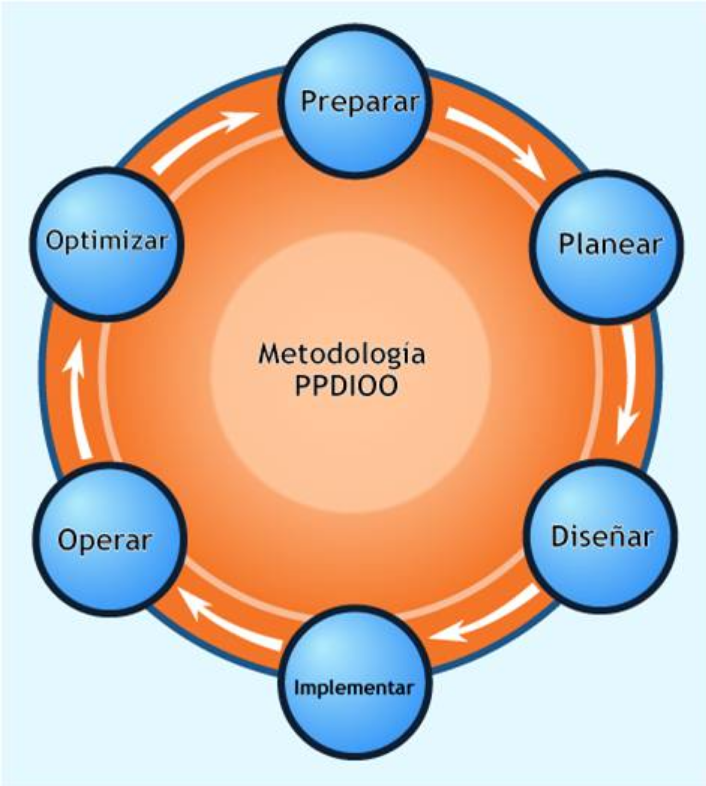
\includegraphics[width=0.5\linewidth]{images/capitulo3/PPDIOO.png}
    \caption{\centering Metodología PPDIOO \cite{PPDIOO}.}
    \label{fig:PPDIOO}
\end{figure}



\subsubsection{Planificación}

En esta fase inicial, se definen los objetivos y especificaciones del nodo sensor. Se identifican los componentes necesarios, que incluyen un sensor de CO\(_2\), un microcontrolador para el procesamiento de datos, y un módulo de comunicación LoRa para el envío de los datos al gateway. También se establecen los requisitos de transmisión, frecuencia de muestreo (configurable) y los umbrales de alerta para la detección de niveles elevados de CO\(_2\).

\subsubsection{Preparación}

Durante la preparación, se lleva a cabo la adquisición de los componentes y se realiza una evaluación de su compatibilidad y consumo energético. Se configura un entorno de desarrollo adecuado y se establecen conexiones de prueba entre el sensor y el microcontrolador, garantizando que el módulo LoRa pueda transmitir adecuadamente los datos generados por el sensor.

\subsubsection{Diseño}

El diseño abarca tanto el esquema de conexiones físicas del nodo sensor como la estructura del código que gestionará las lecturas del sensor. Aquí se diseña el algoritmo que leerá los datos de CO\(_2\), procesará y enviará las lecturas mediante LoRa. Se definen las configuraciones para asegurar una transmisión óptima de los datos y se diseñan métodos de verificación para validar los niveles de CO\(_2\) y activar la transmisión en tiempo real hacia el gateway.

\subsubsection{Implementación}

En la fase de implementación, se ensamblan los componentes electrónicos y se carga el código en el microcontrolador para la captura y transmisión de datos. Se llevan a cabo pruebas de comunicación entre el nodo y el gateway para asegurar que los datos se envían correctamente y que el módulo LoRa funciona de acuerdo con los requisitos establecidos.

\subsubsection{Operación}

Una vez implementado, el nodo sensor se coloca en condiciones de operación para la lectura continua de niveles de CO\(_2\) en el entorno. Esta fase implica una prueba prolongada del nodo para garantizar su rendimiento y la consistencia en la transmisión de datos hacia el gateway bajo diferentes condiciones ambientales.

\subsubsection{Optimización}

Finalmente, la fase de optimización contempla ajustes en la configuración de muestreo y transmisión para optimizar el consumo energético y mejorar la precisión de las lecturas. Se realizan actualizaciones en el código y en la calibración del sensor, de ser necesario, para asegurar que el nodo opere de manera estable y eficiente.


















\section{Desarrollo de la aplicación web}

\subsection{Estudio de requisitos}

\subsubsection{Interfaz de Usuario (Frontend)}

\begin{figure}[H]
    \centering
    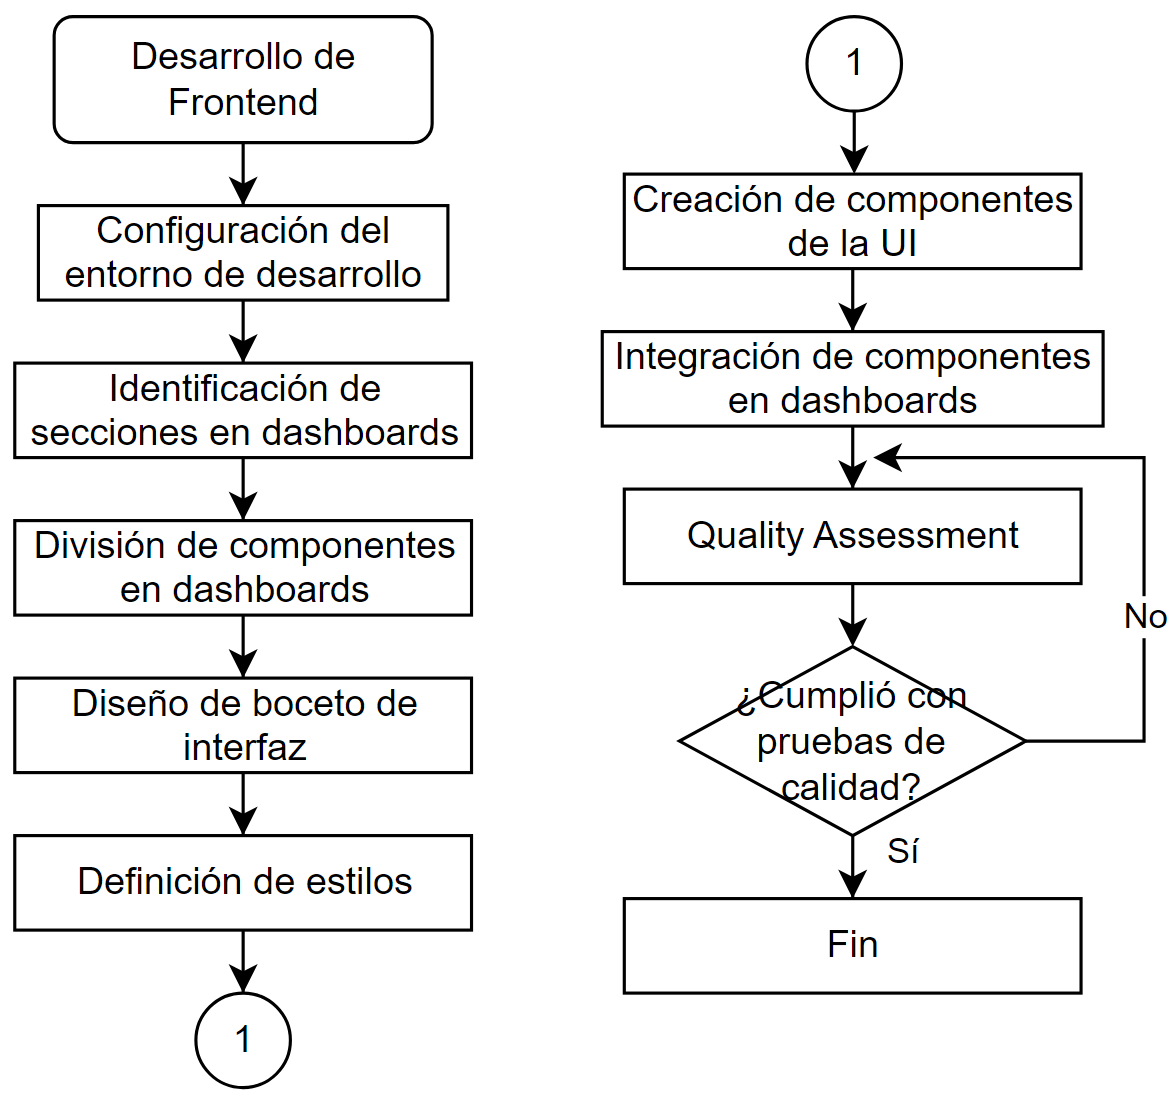
\includegraphics[width=0.6\linewidth]{images//capitulo3/DF_frontend.png}
    \caption{Diagrama de flujo para el desarrollo Frontend}
    \label{fig:DF_frontend}
\end{figure}

En la figura \ref{fig:DF_frontend} se observa la metodología seguida para del desarrollo del frontend de la aplicación web de Monitoreo. En cuanto al paso de evaluación de cualidad (QA: Quality Asessment), consiste en realizar una variedad de pruebas para asegurar el adecuado funcionamiento de la aplicación, cuyos principales focos de atención son los siguientes:

\begin{itemize}
    \item Correcciónes gramaticales.
    \item Bugs y malfuncionamientos en ciertas acciones de la aplicación.
    \item Configuraciones incompletas.
\end{itemize}


Así mismo, la página web cuenta con dos páginas que funcionan como dashboards. La primera es una landing page en la cual se detallan los datos más relevantes en la aplicaciónl, la segunda es una vista detallada para cada uno de los sensores. Las principales funciones de cada una se detallan a continuación.



\begin{itemize}
    \item \textbf{Landing page (Dashboard)}:
          \begin{itemize}
              \item Mostrar las últimas lecturas de CO\(_2\) de tres sensores en tiempo real.
              \item Incluir detalles de la ubicación de cada sensor.
              \item Visualizar las alertas cuando los valores de CO\(_2\) superen el umbral permitido (mediante ventanas emergentes y sonidos de alerta).
          \end{itemize}

    \item \textbf{Vista de Detalle de Sensor}:
          \begin{itemize}
              \item Mostrar información detallada de cada sensor, como el nombre y la ubicación.
              \item Incluir un gráfico interactivo con las lecturas de CO\(_2\) de las últimas 8 horas.
              \item Acceso desde un menú lateral que permite la navegación entre sensores.
          \end{itemize}
\end{itemize}

\subsubsection{Operaciones entre Frontend y Backend}

\begin{itemize}
    \item El frontend debe realizar solicitudes HTTP al backend para recibir actualizaciones de datos de los sensores en tiempo real.
    \item El backend enviará datos actualizados al frontend cada vez que haya una nueva lectura registrada.
    \item Cuando los datos de CO\(_2\) superen el umbral configurado, el backend enviará una señal de alerta que el frontend deberá presentar visual y sonoramente.
    \item El frontend permitirá la consulta histórica de lecturas de CO\(_2\) de cada sensor para su representación en los gráficos.
\end{itemize}

\subsubsection{Interacción con el Mega Gateway Kona}

\begin{itemize}
    \item El mega gateway Kona recibirá los datos de los sensores mediante comunicación LoRa y los enviará al backend utilizando el protocolo MQTT.
    \item El backend debe estar configurado para recibir y procesar mensajes MQTT enviados por el mega gateway Kona.
    \item Los datos recibidos desde el mega gateway Kona deben almacenarse en una base de datos SQL para su posterior visualización y consulta histórica.
    \item En caso de que el mega gateway envíe lecturas que superen el umbral, el backend debe activar el sistema de alertas.
\end{itemize}

\subsubsection{Requisitos de Almacenamiento y Persistencia de Datos}

\begin{itemize}
    \item Los datos de lectura de los sensores deben almacenarse en una base de datos SQL para permitir consultas en tiempo real y acceso a registros históricos.
    \item La base de datos debe registrar la fecha, hora, ubicación y nivel de CO\(_2\) de cada lectura.
    \item Los datos históricos deben poder ser visualizados por el usuario a través de gráficos en la interfaz de detalle de cada sensor.
\end{itemize}









\subsection{Selección de la arquitectura de software}

\begin{table}[h!]
    \centering
    \renewcommand{\arraystretch}{1.5}
    \caption{Comparación de Arquitecturas de Software para Aplicaciones de Monitoreo IoT \cite{software_arquitectura}}
    \label{tabla:software_arquitecturas}
    \begin{tabular}{|p{3cm}|p{2.5cm}|p{2.8cm}|p{2.5cm}|p{3cm}|}
        \hline
        \textbf{Arquitectura}   & \textbf{Escalabilidad}                                                                          & \textbf{Facilidad de Implementación}                                                           & \textbf{Manejo de Datos en Tiempo Real}                                                                & \textbf{Capacidad de Procesamiento}                                                                        \\ \hline
        \textbf{Por capas}      & Moderada: adecuada para aplicaciones pequeñas y medianas                                        & Alta: diseño claro y comúnmente usado en frameworks como ASP.NET y Django                      & Limitada: requiere de modificaciones para soporte en tiempo real                                       & Distribución de lógica de negocio en el backend; buena para procesamiento en servidor                      \\ \hline
        \textbf{Microservicios} & Muy alta: ideal para aplicaciones grandes y escalables, permite añadir servicios independientes & Moderada: requiere experiencia en la gestión de múltiples servicios, comunicación y despliegue & Muy buena: servicios independientes pueden manejar eventos en tiempo real                              & Procesamiento distribuido: cada servicio maneja una funcionalidad específica, óptimo para alto rendimiento \\ \hline
        \textbf{Serverless}     & Alta: escalabilidad automática y flexible, óptima para aplicaciones con carga variable          & Alta: simplifica la implementación al no requerir gestión de servidores                        & Buena: respuesta en tiempo real gestionada por eventos; adecuado para procesamiento en base a umbrales & Limitada al evento y tiempo de ejecución; más eficiente para tareas eventuales o de corta duración         \\ \hline
    \end{tabular}
\end{table}

Se decidió que la arquitectura por capas es ideal para este trabajo de investigación, dado su enfoque accesible, escalable y educativo, adecuado para el monitoreo IoT, ya que ofrece una estructura clara y modular que facilita el aprendizaje práctico de los estudiantes de cada componente en el desarrollo web. La separación en Modelo, Vista y Controlador permite a los estudiantes entender el flujo de datos desde la captura de los sensores hasta la visualización en tiempo real, y aprender de manera segmentada las responsabilidades de cada capa.

Además, la arquitectura por capas es escalable para aplicaciones de mediana complejidad, por lo que, a medida que el proyecto crezca (añadiendo sensores o funciones adicionales), podrá expandirse sin una reestructuración significativa. Su compatibilidad con frameworks educativos, como ASP.NET, el cual es utilizado para este trabajo, facilita la implementación y permite que los estudiantes se enfoquen en la lógica de negocio y el diseño de la interfaz sin la complejidad de arquitecturas más avanzadas.
\FloatBarrier






\subsection{Desarrollo del Frontend}

\subsubsection{Selección de tecnologías de diseño}
\begin{table}[h!]
    \centering
    \renewcommand{\arraystretch}{1.5}
    \caption{Comparación de Tecnologías Frontend para Aplicaciones de Monitoreo IoT}
    \label{tabla:comparativa}
    \begin{tabular}{|p{2.1cm}|p{2cm}|p{2.5cm}|p{2.5cm}|p{2.5cm}|p{3.7cm}|}
        \hline
        \textbf{Tecnología}        & \textbf{Facilidad de Uso}                   & \textbf{Rendimiento}                                          & \textbf{Soporte de Componentes de Visualización}         & \textbf{Escalabilidad}                                & \textbf{Enfoque}                                                                                                              \\ \hline
        \textbf{React}             & Alta: gran documentación y comunidad        & Alto, gracias a su DOM virtual optimizado                     & Amplio: compatible con bibliotecas como Chart.js y D3.js & Alta: compatible con arquitecturas modulares          & Creado para construir interfaces de usuario y gestionar el estado de aplicaciones de una sola página (SPA)                    \\ \hline
        \textbf{Vue.js}            & Muy alta: curva de aprendizaje rápida       & Moderado-Alto: buen manejo de cambios                         & Amplio: compatible con bibliotecas gráficas              & Moderado: adecuado para proyectos pequeños-medianos   & Enfoque progresivo, diseñado para ser adaptable y escalable según las necesidades del proyecto                                \\ \hline
        \textbf{Angular}           & Media: curva de aprendizaje más pronunciada & Alto: rendimiento robusto en aplicaciones grandes             & Muy amplio: incluye gráficos y componentes integrados    & Alta: ideal para proyectos grandes y escalables       & Framework completo orientado a aplicaciones empresariales de gran tamaño y aplicaciones SPA complejas                         \\ \hline
        \textbf{Svelte}            & Muy alta: sintaxis intuitiva y directa      & Muy alto: menos carga de procesamiento en tiempo de ejecución & Moderado: soporte de bibliotecas externas                & Moderado-Alto: más adecuado para aplicaciones ligeras & Diseño enfocado en la eficiencia, compila código en tiempo de desarrollo para optimizar el rendimiento en tiempo de ejecución \\ \hline
        \textbf{Blazor (para C\#)} & Media: requiere familiaridad con .NET       & Alto: ejecuta WebAssembly                                     & Moderado: integrable con bibliotecas .NET                & Alta: conveniente para aplicaciones basadas en .NET   & Orientado a la ejecución de aplicaciones .NET en el navegador usando WebAssembly                                              \\ \hline
    \end{tabular}
\end{table}
\FloatBarrier


Dado que el trabajo de investigación tiene un enfoque educativo y como objetivo principal establecer un flujo de trabajo sencillo para estudiantes, se considera que React es la opción más adecuada para la aplicación de monitoreo IoT. Esto debido a que permite la creación de componentes reutilizables, manteniendo un desarrollo ágil y modular, lo cual es prioritario para que el proyecto sea replicable y fácil de comprender en un entorno educativo, mientras que, a su vez, da margen suficiente para que los estudiantes puedan ajustar la aplicación en torno a sus necesidades específicas y explorar sus propios conceptos.







\subsubsection{Diseño de componentes}

A continuación se presentan los componentes creados e implementados en el diseño, tanto en el dashboard de la landing page, así como en la página de detalle de cada sensor, y la página de configuración del administrador. El código para estos componentes se puede visualizar en el anexo \ref{an:componentes_front}.

\begin{itemize}

    \item \texttt{Sidebar.tsx}: Menú lateral de navegación que permite acceder rápidamente a diferentes secciones de la aplicación, como el Dashboard, detalles de sensores, configuración y ayuda. Incluye iconos para mejorar la usabilidad y el diseño.

    \item \texttt{SensorOverview.tsx}: Muestra un resumen en tiempo real del estado de los sensores de CO\(_2\). Cada sensor tiene su propia tarjeta con información sobre el nivel actual de CO\(_2\), ubicación, estado (normal, elevado, crítico) y última actualización.

    \item \texttt{ComparativeChart.tsx}: Componente que muestra una gráfica comparativa de los niveles de CO\(_2\) de varios sensores a lo largo del tiempo. Permite visualizar las tendencias de CO\(_2\) para cada sensor y ayuda a identificar patrones o picos.

    \item \texttt{Filters.tsx}: Card que permite seleccionar el período de tiempo (última hora, últimas 3 horas, etc.) para filtrar los datos que se muestran en la gráfica comparativa (\texttt{ComparativeChart}). Incluye un selector desplegable para ajustar el rango de tiempo.

    \item \texttt{Statistics.tsx}: Card que muestra las estadísticas generales de los sensores, como el nivel promedio de CO\(_2\), el máximo alcanzado, el tiempo total en alerta y el número de alertas generadas. Está diseñado para adaptarse a la altura de su contenido y optimizar el uso del espacio.

    \item \texttt{AlertHistory.tsx}: Card que muestra un historial de alertas, con información sobre la hora de cada alerta y el nivel de CO\(_2\) registrado. Ayuda a rastrear incidentes pasados y evaluar la frecuencia de las alertas.

    \item \texttt{Alerts.tsx}: Card que muestra las alertas activas en el sistema. Cada alerta tiene información sobre la ubicación, el nivel de CO\(_2\) y el estado (elevado, crítico). Incluye botones de acción (como "Reconocer" y "Silenciar") para gestionar las alertas.

    \item \texttt{CampusMap.tsx} (Opcional): Muestra un mapa del campus con las ubicaciones de los sensores de CO\(_2\) resaltadas. Este componente fue eliminado en la última versión del Dashboard para liberar espacio, pero puede reinsertarse según sea necesario.
\end{itemize}











\subsection{Desarrollo del back end}

\subsubsection{Selección de patrones de diseño}


\begin{landscape}
    \begin{table}[h!]
        \centering
        \renewcommand{\arraystretch}{1.2} % Ajusta la altura de las filas
        \fontsize{9}{10}\selectfont % Reduce aún más el tamaño de la fuente dentro de la tabla
        \caption{Patrones de Diseño Utilizados en el Proyecto \cite{design_patterns} \cite{design_patterns}}
        \label{tabla:patrones-diseno}
        \begin{tabular}{|p{2cm}|p{3cm}|p{3cm}|p{5cm}|p{2cm}|}
            \hline
            \textbf{Patrón de Diseño}                                                                                                                                                      & \textbf{Descripción} & \textbf{Función en el Proyecto} & \textbf{Beneficios} & \textbf{Capa(s) de la Arquitectura} \\ \hline

            \textbf{DTO (Data Transfer Object)}                                                                                                                                            &
            Objeto simple que encapsula datos para transferir entre capas, evitando exponer directamente las entidades del dominio.                                                        &
            Facilita la transferencia de datos de las lecturas de sensores y alertas al frontend, asegurando que solo se transmita la información necesaria.                               &
            \begin{itemize}[leftmargin=*, nosep]
                \item Reduce el acoplamiento entre capas.
                \item Mejora la seguridad al no exponer entidades internas.
                \item Optimiza el rendimiento al transferir solo datos esenciales.
            \end{itemize}                                                                                                         &
            Capa de Aplicación $\leftrightarrow$ Capa de Presentación                                                                                                                                                                                                                                           \\ \hline

            \textbf{Repository Pattern}                                                                                                                                                    &
            Abstracción que maneja las operaciones de acceso a datos, proporcionando una interfaz para realizar operaciones CRUD.                                                          &
            Gestiona la interacción con la base de datos para almacenar y recuperar lecturas de sensores, así como verificar umbrales para generar alertas.                                &
            \begin{itemize}[leftmargin=*, nosep]
                \item Aísla la lógica de acceso a datos de la lógica de negocio.
                \item Facilita la prueba y mantenimiento del código.
                \item Permite cambiar el proveedor de datos sin afectar otras capas.
            \end{itemize}                                                                                                       &
            Capa de Persistencia                                                                                                                                                                                                                                                                                \\ \hline

            \textbf{Entity Framework (ORM)}                                                                                                                                                &
            Herramienta de mapeo objeto-relacional que permite interactuar con la base de datos utilizando modelos de entidad en lugar de consultas SQL directas.                          &
            Simplifica la gestión de la base de datos, permitiendo mapear las lecturas de sensores y alertas a entidades de C\#.                                                           &
            \begin{itemize}[leftmargin=*, nosep]
                \item Reduce la complejidad del acceso a datos.
                \item Facilita la gestión de cambios en el esquema de la base de datos.
                \item Mejora la productividad al eliminar la necesidad de escribir consultas SQL manualmente.
            \end{itemize}                                                                              &
            Capa de Persistencia                                                                                                                                                                                                                                                                                \\ \hline

            \textbf{Service Pattern}                                                                                                                                                       &
            Organiza la lógica de negocio en servicios independientes y reutilizables que encapsulan operaciones específicas.                                                              &
            Centraliza la lógica de procesamiento de datos de sensores, evaluación de umbrales y generación de alertas, manteniendo la lógica de negocio separada de otras preocupaciones. &
            \begin{itemize}[leftmargin=*, nosep]
                \item Promueve la reutilización de código.
                \item Mejora la mantenibilidad y escalabilidad del sistema.
                \item Facilita la implementación de pruebas unitarias.
            \end{itemize}                                                                                                                &
            Capa de Aplicación                                                                                                                                                                                                                                                                                  \\ \hline
        \end{tabular}
    \end{table}
    \FloatBarrier % Evita que las tablas floten por encima de este punto
\end{landscape}
\FloatBarrier














\subsubsection{Desarrollo de REST API}
\begin{figure}
    \centering
    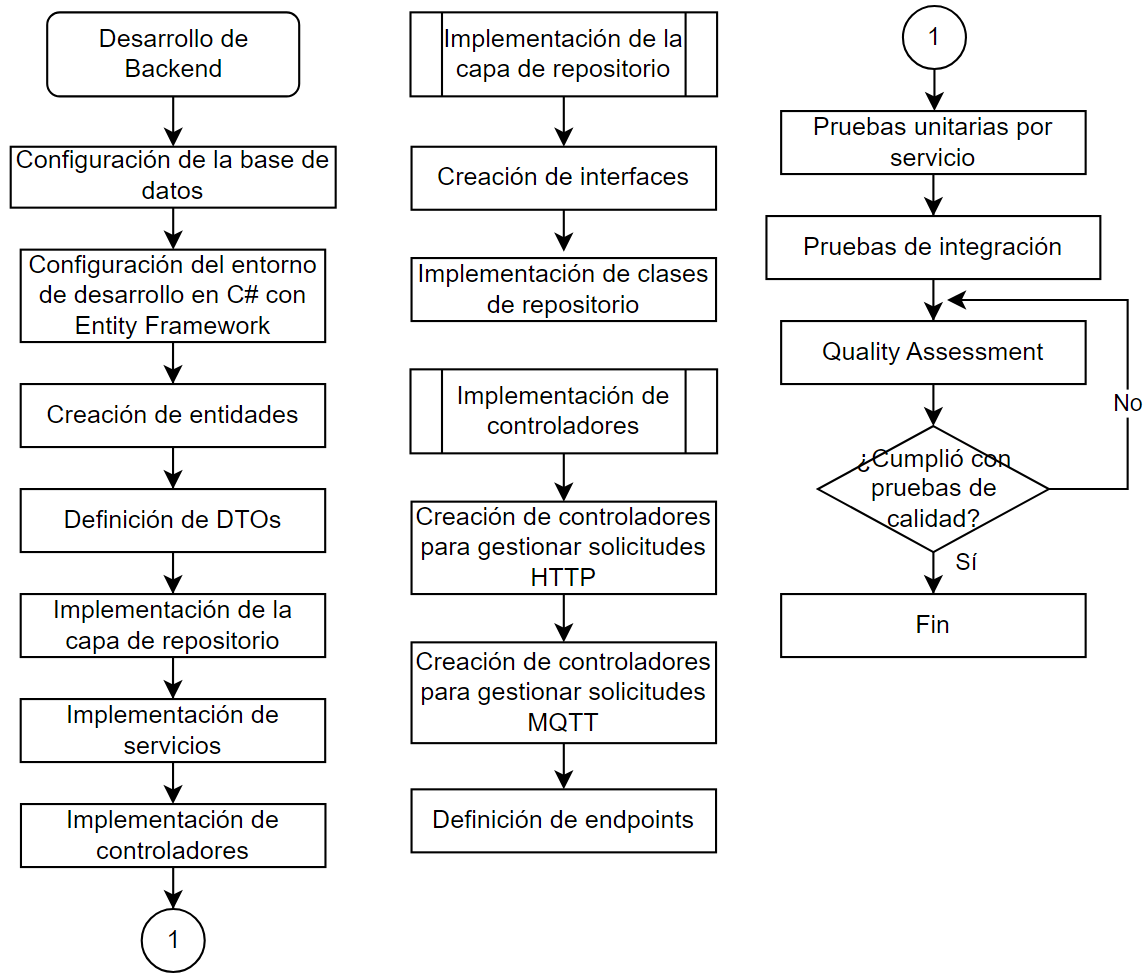
\includegraphics[width=0.8\linewidth]{images/capitulo3/DF_backend.png}
    \caption{Diagrama de flujo del desarrollo de Backend.}
    \label{fig:df_backend}
\end{figure}


El desarrollo backend sigue una arquitectura de capas en la que cada sección tiene un rol específico para gestionar las operaciones de datos de los sensores. La configuración inicial incluye la base de datos y el entorno en C\# con Entity Framework, permitiendo un acceso simplificado a MySQL mediante mapeo de objetos.

Las entidades representan las tablas en la base de datos, y los DTOs permiten transferir datos de forma controlada entre capas, protegiendo la estructura de la base de datos. La capa de repositorio usa el \textit{Repository Pattern} para manejar las operaciones \textit{CRUD} de manera aislada. La capa de servicios aplica la lógica de negocio, como verificar los umbrales de CO\(_2\) y gestionar alertas. Finalmente, los controladores gestionan las solicitudes \texttt{HTTP} y \texttt{MQTT}, proporcionando los datos al frontend mediante endpoints bien definidos.

Las pruebas unitarias e integración aseguran la calidad y funcionamiento del sistema antes del despliegue. El proceso de Quality Assessment verifica que todos los componentes cumplen con los estándares de calidad antes de finalizar el desarrollo.



\section{Desarrollo del nodo sensor}

\subsection{Selección de la tecnología de comunicación}

Antes de definir los componentes electrónicos específicos del nodo sensor, es fundamental seleccionar la tecnología de comunicación inalámbrica que mejor se adapte a los requerimientos del proyecto. En la Tabla \ref{tabla:comparativa_comunicacion} se presenta una comparativa entre las principales tecnologías IoT disponibles en el mercado, evaluadas según los criterios de diseño específicos de esta investigación.

\begin{landscape}
    \begin{table}[h!]
        \centering
        \renewcommand{\arraystretch}{1.3}
        \fontsize{9}{10}\selectfont
        \caption{Comparación de Tecnologías de Comunicación Inalámbrica para Nodos Sensores}
        \label{tabla:comparativa_comunicacion}
        \begin{tabular}{|p{2.5cm}|p{2.5cm}|p{2cm}|p{2cm}|p{2.5cm}|p{2.5cm}|p{4.5cm}|p{2cm}|}
            \hline
            \textbf{Característica}     & \textbf{LoRa}                & \textbf{Zigbee}           & \textbf{Wi-Fi}           & \textbf{Bluetooth (BLE)}        & \textbf{NB-IoT / LTE-M (Celular IoT)} & \textbf{Criterio de Diseño (Lo que busca tu Proyecto)}                                                            & \textbf{Mejor Opción}                       \\ \hline
            \textbf{Frecuencia}         & Sub-GHz (915 MHz en Perú)    & 2.4 GHz                   & 2.4 GHz y 5 GHz          & 2.4 GHz                         & Bandas Licenciadas LTE                & Se busca una frecuencia libre (ISM) y legal en Perú, preferiblemente Sub-GHz para evitar interferencia en 2.4GHz. & LoRa (915 MHz)                              \\ \hline
            \textbf{Alcance (Urbano)}   & Alto (1--5 km con obstáculos) & Bajo (10--100 m)           & Bajo (30--100 m)         & Muy Bajo ($<$10 m)                & Muy Alto ($>$5 km)                          & Se busca cubrir múltiples laboratorios en un campus universitario con un solo gateway central.                    & LoRa / Wi-Fi (ya se cuenta con repetidores) \\ \hline
            \textbf{Consumo Energía}    & Muy Bajo ($\sim$40 mA TX, pero ciclo de trabajo $<$1\%) & Bajo ($\sim$30 mA TX, pero mayor overhead en red mesh) & Alto ($\sim$200 mA TX, conexión constante $>$1 mA) & Muy Bajo ($<$15 mA TX, ráfagas muy cortas) & Medio ($\sim$200 mA TX, pero usa PSM de $\sim$3 $\mu$A)                            & Se busca que los nodos sensores puedan funcionar con baterías durante meses sin mantenimiento.                    & LoRa / BLE                                  \\ \hline
            \textbf{Tasa de Datos}      & Muy Baja (0.3--50 kbps)          & Baja (250 kbps)           & Muy Alta ($>$50 Mbps)      & Media (1--2 Mbps)                & Baja ($<$250 kbps)                            & Se busca enviar solo unos pocos bytes (valor de CO$_2$) cada varios minutos.                                      & LoRa                                        \\ \hline
            \textbf{Penetración Muros}  & Muy Alta (Link Budget $\sim$157 dB) & Baja ($\sim$104 dB) & Baja ($\sim$100 dB) & Muy Baja ($\sim$90 dB) & Muy Alta ($\sim$164 dB) & Se busca atravesar muros de concreto armado densos típicos de laboratorios y aulas.                               & LoRa / NB-IoT                               \\ \hline
            \textbf{Costo del Nodo}     & Medio (\$5--\$15)              & Muy Bajo (\$3--\$10)           & Muy Bajo (\$3--\$8)       & Muy Bajo (\$2--\$5)              & Alto (\$15--\$30)                     & Se busca minimizar el costo por nodo sensor para un despliegue de tesis.                                          & Wi-Fi / BLE                                 \\ \hline
            \textbf{¿Necesita Gateway?} & Sí                           & Sí                        & No (Router directo)      & No (Directo a móvil/PC)         & No (Base celular)                     & -                                                                                                                 & LoRa                                        \\ \hline
            \textbf{Costos Operativos}  & Muy Bajos (Nulos, red propia) & Muy Bajos (Nulos, red propia) & Muy Bajos (Nulos, red U) & Muy Bajos (Nulos)               & Altos (Suscripción mensual)           & Se busca un costo mensual cero por tráfico de datos para sostenibilidad.                                          & LoRa / Wi-Fi / Zigbee                       \\ \hline
        \end{tabular}
    \end{table}
\end{landscape}
\FloatBarrier

De acuerdo con el análisis presentado en la Tabla \ref{tabla:comparativa_comunicacion}, la tecnología \textbf{LoRa} destaca como la solución más viable y que mejor cumple con los criterios de diseño del proyecto. Su alcance en zonas urbanas (clasificado como Alto) permite conectar múltiples laboratorios en el campus utilizando un solo gateway, y su muy alta capacidad de penetración de muros resulta indispensable en infraestructuras con concreto armado. Además, opera en la banda libre de 915 MHz, idónea en Perú para evitar la congestión típica de la banda de 2.4 GHz. Un factor decisivo es su muy bajo consumo energético general; aunque su corriente pico de transmisión es comparable a la de tecnologías como Zigbee, la arquitectura de red en estrella de LoRa permite que los nodos sensores permanezcan en reposo profundo la mayor parte del tiempo (ciclo de trabajo inferior al 1\%), evitando el constante enrutamiento de datos y el alto overhead característicos de las redes en malla (mesh). Sumado a sus costos operativos muy bajos (prácticamente nulos al ser red propia), LoRa se convierte en la opción ideal para un despliegue sostenible a largo plazo, a pesar de su muy baja tasa de datos, la cual es suficiente para transmitir lecturas esporádicas de CO$_2$.

\subsection{Gateways comerciales frente a la implementación de gateways personalizados}

Para el despliegue de redes LoRaWAN enfocadas en Internet de las Cosas (IoT), la literatura resalta tres enfoques principales para la capa de borde (Edge): gateways comerciales de grado operador, gateways comerciales de bajo costo (prosumer) y gateways personalizados construidos a medida (Do-It-Yourself o DIY).

Los \textbf{gateways comerciales de grado operador (Carrier-Grade)}, como el Kona Mega Gateway, representan el estándar de infraestructura masiva. Cuentan con multiplexación avanzada para manejar entre 64 y 72 canales simultáneos, erradicando virtualmente las colisiones en el aire \cite{nb_gateway_commercial_1}, y poseen filtros físicos que logran sensibilidades excepcionales de -142 dBm \cite{nb_gateway_commercial_4}. Sin embargo, sus elevados costos (CAPEX) y la inflexibilidad de su ecosistema cerrado los hacen inviables e incompatibles con arquitecturas atípicas requeridas en proyectos universitarios de pequeña escala \cite{nb_gateway_commercial_6, nb_gateway_commercial_7}.

Por otro lado, los \textbf{gateways comerciales de bajo costo (Prosumer)}, como el RAK7268V2 o SenseCAP M2, buscan democratizar el acceso con costos entre \$89 y \$500 USD \cite{nb_gateway_commercial_6}. Integran criptografía robusta en hardware (ATECC608A) y procesadores digitales de señal (DSP) \cite{nb_gateway_prosumer_29}. A pesar de estos beneficios, su limitación a 8 canales físicos genera riesgos de congestión, forzando la dependencia de mecanismos como la Tasa de Datos Adaptativa (ADR) \cite{nb_gateway_prosumer_32, nb_gateway_prosumer_34}, además de incurrir en costos ocultos de importación y periféricos adicionales \cite{nb_gateway_prosumer_41}.

Finalmente, los \textbf{gateways personalizados (Custom/DIY)} se ensamblan acoplando microcontroladores o computadoras de placa única (SBC) a módulos concentradores LoRa o transceptores \cite{nb_gateway_custom_9}. Este enfoque ofrece flexibilidad absoluta de software y control total sobre las rutinas de enrutamiento \cite{nb_gateway_custom_7}. Su principal virtud es la posibilidad de operar en modo ``promiscuo'', lo que permite interactuar con nodos de ultra bajo costo que carecen de la pila LoRaWAN completa, además de reducir dramáticamente el presupuesto de implementación \cite{nb_gateway_custom_10}. Si bien presentan riesgos asociados a la alta complejidad técnica y soporte fragmentado, estos desafíos son coherentes y deseables en el marco de una investigación de tesis en Ingeniería Mecatrónica, donde se busca precisamente el dominio de la integración hardware-software a bajo nivel.

En conclusión, para este proyecto universitario desarrollado en Lima, Perú, se determina la viabilidad técnica y académica de optar por el diseño e implementación de un \textbf{gateway personalizado}. La priorización de la flexibilidad para configurar nodos simples, la reducción contundente del CAPEX y la alineación con los objetivos de diseño embebido respaldan sólidamente esta decisión frente al sobredimensionamiento y rigidez de los equipos comerciales. Esta elección fundamenta, a su vez, la necesidad de una evaluación exhaustiva de microcontroladores y módulos de comunicación para el ensamble tanto del nodo sensor como del gateway.

\subsection{Selección de componentes}

Para determinar los elementos electrónicos y de comunicación que compondrán tanto los nodos sensores como el gateway personalizado, se evalúan las principales alternativas reportadas en la literatura. Dado que el proyecto requiere viabilidad para un prototipado realista y replicable en el entorno universitario (Lima, Perú), se han ajustado los criterios de evaluación otorgando un peso preponderante del 35\% a la ``Disponibilidad en el mercado local'' y 30\% a la ``Facilidad de configuración / Abundancia de documentación''. A continuación, se presentan las matrices de evaluación para microcontroladores, módulos LoRa y módulos Wi-Fi.

\subsubsection{Evaluación de Microcontroladores}

Se evaluaron cuatro opciones predominantes:
\begin{itemize}
    \item \textbf{MCU 1: ATmega328P.} Microcontrolador base de Arduino UNO. Su severa limitación de memoria SRAM provoca inestabilidad al intentar implementar una pila LoRaWAN completa \cite{nb_mcu_1, nb_mcu_3}.
    \item \textbf{MCU 2: ESP32.} Microcontrolador de muy bajo costo con conectividad Wi-Fi nativa, altamente versátil para nodos sensores austeros y tareas de enrutamiento en gateways minimalistas \cite{nb_mcu_4, nb_mcu_6}.
    \item \textbf{MCU 3: ESP32-S3.} Variante de doble núcleo, utilizada en gateways comerciales de bajo costo para compilar lógicas de reenvío digital \cite{nb_mcu_6}.
    \item \textbf{MCU 4: Microchip ATECC608A.} Coprocesador criptográfico utilizado para cifrado de hardware, pero que no actúa como unidad de procesamiento general \cite{nb_mcu_8}.
\end{itemize}

\begin{table}[H]
    \centering
    \renewcommand{\arraystretch}{1.5}
    \caption{Evaluación Comparativa de Microcontroladores}
    \label{tabla:evaluacion_mcu}
    \begin{tabular}{|p{4.5cm}|p{1.5cm}|p{1.5cm}|p{1.5cm}|p{1.5cm}|p{1.5cm}|}
        \hline
        \textbf{Criterio de Evaluación} & \textbf{Peso} & \textbf{MCU 1} & \textbf{MCU 2} & \textbf{MCU 3} & \textbf{MCU 4} \\ \hline
        Disponibilidad local & 35\% & 4 (1.40) & 4 (1.40) & 2 (0.70) & 1 (0.35) \\ \hline
        Facilidad de configuración & 30\% & 4 (1.20) & 4 (1.20) & 3 (0.90) & 2 (0.60) \\ \hline
        Capacidad de procesamiento/RAM & 20\% & 1 (0.20) & 3 (0.60) & 4 (0.80) & 2 (0.40) \\ \hline
        Costo & 15\% & 3 (0.45) & 4 (0.60) & 3 (0.45) & 2 (0.30) \\ \hline
        \textbf{Puntaje Total} & \textbf{100\%} & \textbf{3.25} & \textbf{3.80} & \textbf{2.85} & \textbf{1.65} \\ \hline
    \end{tabular}
\end{table}

\subsubsection{Evaluación de Módulos LoRa}

Las alternativas para la capa física de radiofrecuencia (transceptores/concentradores) incluyen:
\begin{itemize}
    \item \textbf{LoRa 1: Ebyte E220-900T30D.} Transceptor UART de bajo costo basado en el chip LLCC68, ideal para nodos y gateways monocanal simples, aunque requiere que la estructura de red sea gestionada por software \cite{nb_lora_1}.
    \item \textbf{LoRa 2: RAKwireless RAK2287.} Módulo concentrador impulsado por el chip SX1302 con escudo EMI, excelente para gateways multicanal robustos \cite{nb_lora_13}.
    \item \textbf{LoRa 3: Seeed Studio Wio-WM1302.} Tarjeta concentradora SX1302 con certificaciones industriales, optimizada en consumo y costo \cite{nb_lora_13_seeed}.
    \item \textbf{LoRa 4: Dragino PG1302.} Módulo tipo Pi HAT orientado a presupuestos ajustados, pero con soporte técnico limitado \cite{nb_lora_13_dragino}.
\end{itemize}

\begin{table}[H]
    \centering
    \renewcommand{\arraystretch}{1.5}
    \caption{Evaluación Comparativa de Módulos LoRa}
    \label{tabla:evaluacion_lora}
    \begin{tabular}{|p{4.5cm}|p{1.5cm}|p{1.5cm}|p{1.5cm}|p{1.5cm}|p{1.5cm}|}
        \hline
        \textbf{Criterio de Evaluación} & \textbf{Peso} & \textbf{LoRa 1} & \textbf{LoRa 2} & \textbf{LoRa 3} & \textbf{LoRa 4} \\ \hline
        Disponibilidad local & 35\% & 4 (1.40) & 1 (0.35) & 1 (0.35) & 2 (0.70) \\ \hline
        Facilidad de configuración & 30\% & 4 (1.20) & 3 (0.90) & 3 (0.90) & 2 (0.60) \\ \hline
        Capacidad multicanal / SNR & 20\% & 2 (0.40) & 4 (0.80) & 4 (0.80) & 3 (0.60) \\ \hline
        Costo & 15\% & 4 (0.60) & 2 (0.30) & 3 (0.45) & 3 (0.45) \\ \hline
        \textbf{Puntaje Total} & \textbf{100\%} & \textbf{3.60} & \textbf{2.35} & \textbf{2.50} & \textbf{2.35} \\ \hline
    \end{tabular}
\end{table}

\subsubsection{Evaluación de Módulos Wi-Fi}

Para la transmisión del lado del gateway o nodos que cuenten con enlace directo al servidor:
\begin{itemize}
    \item \textbf{Wi-Fi 1: Módulo Wi-Fi 4 Estándar (802.11 b/g/n).} Componente externo genérico presente en gateways comerciales, idóneo para 2.4 GHz y entornos urbanos \cite{nb_wifi_16}.
    \item \textbf{Wi-Fi 2: Wi-Fi Nativo ESP32.} Circuitería embebida en el encapsulado del microcontrolador ESP32. Provee un puente directo e ininterrumpido al enrutador sin requerir hardware físico adicional \cite{nb_mcu_4, nb_mcu_6}.
    \item \textbf{Wi-Fi 3: Wi-Fi 5 de Orange Pi Zero 3.} Módulo embebido en la SBC, con alta conectividad para arquitecturas de Edge Computing.
    \item \textbf{Wi-Fi 4: Wi-Fi 5 de Raspberry Pi 4.} Integración inalámbrica de alta velocidad apta para albergar bases de datos locales complejas.
\end{itemize}

\begin{table}[H]
    \centering
    \renewcommand{\arraystretch}{1.5}
    \caption{Evaluación Comparativa de Soluciones Wi-Fi}
    \label{tabla:evaluacion_wifi}
    \begin{tabular}{|p{4.5cm}|p{1.5cm}|p{1.5cm}|p{1.5cm}|p{1.5cm}|p{1.5cm}|}
        \hline
        \textbf{Criterio de Evaluación} & \textbf{Peso} & \textbf{Wi-Fi 1} & \textbf{Wi-Fi 2} & \textbf{Wi-Fi 3} & \textbf{Wi-Fi 4} \\ \hline
        Disponibilidad local & 35\% & 3 (1.05) & 4 (1.40) & 2 (0.70) & 3 (1.05) \\ \hline
        Facilidad de configuración & 30\% & 3 (0.90) & 4 (1.20) & 3 (0.90) & 4 (1.20) \\ \hline
        Ancho de banda & 20\% & 3 (0.60) & 2 (0.40) & 4 (0.80) & 4 (0.80) \\ \hline
        Integración y tamaño & 15\% & 2 (0.30) & 4 (0.60) & 3 (0.45) & 2 (0.30) \\ \hline
        \textbf{Puntaje Total} & \textbf{100\%} & \textbf{2.85} & \textbf{3.60} & \textbf{2.85} & \textbf{3.35} \\ \hline
    \end{tabular}
\end{table}

\subsubsection{Justificación Cualitativa de Resultados}

Con base en la evaluación de los tres dominios presentados, la selección final converge de manera natural y transparente hacia el ecosistema del \textbf{ESP32 (MCU 2 y Wi-Fi 2)} en conjunto con el \textbf{módulo Ebyte E220-900T30D (LoRa 1)}.

Debido a que el proyecto se contextualiza como un desarrollo universitario en Lima y se ha priorizado el modelo de diseño "Custom/DIY", la ponderación asignada a la "Disponibilidad en el mercado local" y la "Facilidad de configuración" ha sido decisiva. El ESP32 lidera sólidamente frente a alternativas limitadas como el ATmega328P o escasas como el ESP32-S3, brindando memoria holgada para gestionar las rutinas de transmisión e integrando sin costo adicional ni ocupación de espacio físico una interfaz Wi-Fi completamente funcional.

Por otro lado, aunque los concentradores multicanal basados en el SX1302 (como el RAK2287) presentan un puntaje técnico superior en capacidad de radio, su nula disponibilidad en el mercado local, sus altos aranceles de importación y su exigente curva de aprendizaje penalizan severamente su puntaje final. En contraste, el módulo E220-900T30D (915 MHz) domina el mercado nacional peruano de prototipado, resulta extremadamente accesible y es plenamente compatible con el ESP32 mediante su interfaz serial UART. Esta sinergia ESP32 + E220-900T30D permite construir nodos y un gateway base altamente viables, respaldados por una inmensa comunidad técnica que garantiza el cumplimiento de los objetivos de la tesis.

\subsection{Criterios Normativos para la Ubicación Espacial de los Nodos Sensores}

Para garantizar la fiabilidad y representatividad de las mediciones de dióxido de carbono (CO$_2$) en espacios universitarios, como laboratorios y aulas, es imperativo fundamentar la instalación física de los nodos sensores en normativas y estándares internacionales reconocidos. Un posicionamiento incorrecto puede derivar en lecturas sesgadas o la aparición de puntos ciegos. A partir de la revisión de literatura, se detallan los siguientes criterios estandarizados adoptados para este proyecto:

\subsubsection{Altura de Colocación Respecto a la Zona de Respiración}
Las normativas convergen en que los sensores deben situarse de manera que capturen el aire en la ``zona de respiración'' típica de los ocupantes. El estándar \textit{RESET} y el estándar \textit{WELL} recomiendan el montaje vertical en paredes a una altura comprendida entre 1.1 y 1.7 metros (o de 900 a 1800 mm) desde el nivel del suelo \cite{reset_standard_v2, well_performance_guidebook}. Por su parte, la normativa ASHRAE 62.1-2022 define esta zona de respiración en un rango similar, desde 75 hasta 1800 mm de altura \cite{ashrae_62_1_2022}. En el contexto específico de entornos educativos y de cuidado infantil, el gobierno británico aconseja de forma práctica posicionar los sensores a la altura de las mesas o de las cabezas de los estudiantes cuando se encuentran sentados \cite{gov_uk_ventilation_education}. 

\subsubsection{Distancia Mínima a Fuentes de Ventilación y Aperturas}
La proximidad a flujos de aire directo puede alterar las mediciones reales del ambiente, generando subestimaciones del riesgo. En este sentido, el estándar \textit{RESET} indica una separación mínima de 5 metros respecto a ventanas operables, filtros y difusores de aire fresco \cite{reset_standard_v2}. En caso de que el espacio sea demasiado pequeño, el sensor no debe instalarse a una distancia menor a la mitad del ancho de la habitación respecto a las ventanas. Asimismo, normativas como \textit{WELL} y \textit{RESET} dictaminan un alejamiento mínimo de 1 metro de puertas interiores, ventanas, sistemas mecánicos de suministro de aire y cualquier fuente significativa de calor o frío \cite{well_performance_guidebook, reset_standard_v2}. En el caso de puertas que den al exterior, se requieren precauciones adicionales, debiendo mantener una separación de 3 a 5 metros para evitar corrientes de aire irregulares al abrirse \cite{well_performance_guidebook}. El gobierno británico también es explícito en este punto, recomendando alejar los sensores de salidas de ventilación \cite{gov_uk_ventilation_education}.

\subsubsection{Posicionamiento Estratégico y Representatividad Espacial}
Para que las lecturas sean útiles en un sistema de mitigación, los monitores deben estar instalados de manera representativa. \textit{RESET} exige que se ubiquen centralmente en el espacio \cite{reset_standard_v2}. Además, para evitar lecturas distorsionadas causadas por la exhalación directa de una persona, el gobierno británico aconseja colocar los sensores a una distancia de al menos 0.5 metros de cualquier ocupante \cite{gov_uk_ventilation_education}. Como regla general para aulas escolares típicas, un único sensor ubicado según estas directrices es suficiente para obtener medidas precisas de la sala completa \cite{gov_uk_ventilation_education}. En casos de ambientes más amplios y diáfanos, \textit{WELL} permite utilizar un solo monitor por cada 2500 metros cuadrados si existen evidencias de un volumen de aire bien mezclado sin puntos ciegos \cite{well_performance_guidebook}. De forma excepcional, \textit{WELL} habilita la instalación horizontal en techos solo si su altura es inferior a 3.7 metros y se demuestra una mezcla homogénea de aire \cite{well_performance_guidebook}, sin embargo, el enfoque central en la zona de respiración montada en pared es el más apropiado para las aulas universitarias del proyecto.


\subsubsection{Definición de Parámetros de Instalación}
Con base en las normativas expuestas, se ha consolidado un conjunto de reglas precisas para la instalación física de los nodos sensores en los espacios evaluados de la universidad. Estos parámetros buscan un equilibrio entre el cumplimiento de los estándares internacionales (ASHRAE, RESET, WELL) y las particularidades arquitectónicas de las aulas universitarias, garantizando mediciones consistentes y libres de sesgos. En la Tabla \ref{tabla:criterios_instalacion} se resumen las recomendaciones de la literatura frente a los valores definitivos seleccionados para el despliegue de esta tesis.

\begin{table}[H]
    \centering
    \renewcommand{\arraystretch}{1.5}
    \caption{Selección de Criterios para la Instalación de Nodos Sensores de CO$_2$}
    \label{tabla:criterios_instalacion}
    \begin{tabular}{|p{4cm}|p{5.5cm}|p{4.5cm}|}
        \hline
        \textbf{Criterio de Instalación} & \textbf{Recomendación de la Literatura} & \textbf{Valor Seleccionado para el Proyecto} \\ \hline
        Altura de colocación & 1.1 a 1.7 m (RESET, WELL); 0.75 a 1.8 m (ASHRAE); Altura de cabeza sentado (GOV.UK) & \textbf{1.2 metros} (Altura promedio de respiración de estudiantes sentados) \\ \hline
        Distancia a fuentes de aire directo (ventanas, difusores) & 5 m ideal, o mínimo mitad del ancho de la habitación (RESET) & \textbf{$\geq$ 2.5 metros} (Adaptado al tamaño de las aulas universitarias) \\ \hline
        Distancia a puertas y ventanas cerradas & Mínimo 1 m (WELL, RESET) & \textbf{1.5 metros} \\ \hline
        Distancia a puertas exteriores & 3 a 5 metros (WELL) & \textbf{$\geq$ 4 metros} \\ \hline
        Distancia a ocupantes & Mínimo 0.5 metros (GOV.UK) & \textbf{1 metro} de separación del escritorio más cercano \\ \hline
        Posicionamiento espacial & Central en la habitación (RESET) o en techo si H $<$ 3.7 m y aire mixto (WELL) & \textbf{Pared central}, sin interferencias u obstáculos directos \\ \hline
    \end{tabular}
\end{table}

La justificación de los valores definidos en la Tabla \ref{tabla:criterios_instalacion} responde directamente a la dinámica del flujo de aire y al comportamiento habitual en las aulas. Al seleccionar una altura de 1.2 metros, se asegura que las lecturas reflejen de manera precisa la concentración de dióxido de carbono que los estudiantes están inhalando mientras permanecen sentados durante las clases teóricas, evitando la recolección de aire estancado a nivel del suelo o bolsas de calor cerca del techo. Por otro lado, establecer distancias mínimas estrictas frente a ventanas operables (2.5 metros) y puertas (1.5 metros) previene que corrientes puntuales de aire fresco diluyan artificialmente las mediciones, lo que podría retrasar la activación del sistema de mitigación predictiva. Finalmente, mantener una distancia prudente de 1 metro respecto a los estudiantes y centralizar los sensores en las paredes laterales permite evaluar el estado volumétrico real de la masa de aire del aula, garantizando una caracterización homogénea y confiable del entorno evaluado.

\newpage
\section{Configuración del gateway}
Para la configuración del gateway Kona Mega, primero se debe confirmar que tanto la computadora, desde donde se enviará la configuración, y el gateway estén en la misma red. Se pueden emplear 2 herramientas. Por un lado, se tiene la opción de utilizar una consola para comunicarse con el dispositivo via SSH (Secure Shell). Esto puede realizarse ya sea en el sistema operativo (OS: Operative System) Linux, el cual cuenta con una consola SSH preinstalada, así como una serie de comandos que pueden agilizar la interacción con el gateway durante la configuración; o también se pueden utilizar aplicaciones como PuTTY para la comunicación via SSH. Por otro lado, se puede emplear la aplicacion Kona Field Tool (KonaFT), la cual fue la empleada en este proyecto. Esta herramienta no solo permite realizar las configuraciones del gateway mediante una interfaz gráfica de usuario (GUI: Graphic User Interface), sino también, identificar la dirección IP de todos los dispositivos TekTelic conectados a la misma red que la computadora en la que está instalada el programa. El proceso de idetificación y configuración del gateway sigue el siguiente flujo mostrado en la figura \ref{fig:DF_gateway}.


\begin{figure}
    \centering
    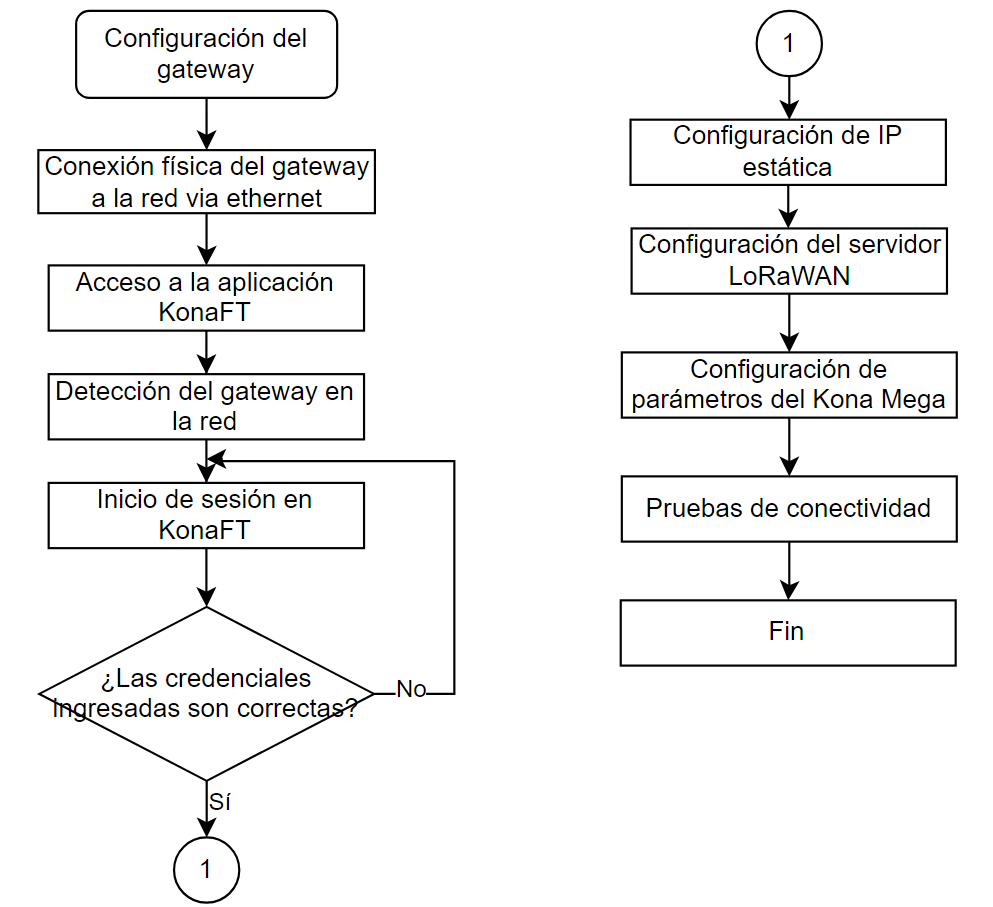
\includegraphics[width=0.8\linewidth]{images/capitulo3/DF_gateway.png}
    \caption{Diagrama de flujo de la configuración del gateway Kona Mega.}
    \label{fig:DF_gateway}
\end{figure}




\newpage
\section{Desarrollo del subsistema de mitigación activa y control}
En esta sección se presenta el desarrollo del subsistema de mitigación activa y control, incorporado con el propósito de extender la funcionalidad del sistema más allá del monitoreo pasivo de la concentración de CO$_2$. Este subsistema se basa en la actuación automática de ventiladores modulados por PWM, de modo que la ventilación del ambiente pueda ajustarse de acuerdo con las condiciones medidas en tiempo real. Para ello, se considera la definición de requisitos del subsistema, la selección de actuadores y fuente de alimentación, el diseño de la arquitectura de control, el modelado del comportamiento dinámico del CO$_2$ en ambientes interiores y la implementación de controladores PID y Fuzzy. Finalmente, se establecen los criterios de validación experimental para comparar ambas estrategias y determinar su conveniencia dentro del sistema propuesto.




\subsection{Definición de requisitos del subsistema de ventilación}

En esta etapa se establecen los requisitos funcionales y no funcionales del subsistema de ventilación activa, cuyo propósito es contribuir a la reducción de la concentración de CO$_2$ en ambientes interiores a partir de la información proporcionada por el sistema de monitoreo. Para ello, el subsistema debe ser capaz de recibir como entrada la concentración de CO$_2$ medida en tiempo real, compararla con un valor de referencia establecido y generar una acción de control que permita regular la velocidad de los ventiladores mediante señal PWM. Asimismo, el subsistema debe integrarse con la arquitectura general del proyecto, de modo que la etapa de sensado, procesamiento, actuación y visualización funcione de manera coordinada.

Desde el punto de vista funcional, se requiere que el sistema permita la activación automática de la ventilación cuando la concentración de CO$_2$ supere el nivel de referencia definido, así como la modulación de la velocidad de los ventiladores de acuerdo con la estrategia de control implementada. De igual manera, debe registrar variables relevantes para el análisis experimental, tales como la concentración medida, el error respecto al setpoint y la señal de control aplicada. Adicionalmente, el diseño debe permitir la implementación y comparación de distintas estrategias de control, específicamente PID y Fuzzy, a fin de evaluar su desempeño en términos de rapidez de respuesta, estabilidad y capacidad de mitigación.

En cuanto a los requisitos no funcionales, el subsistema debe emplear componentes comerciales de fácil adquisición e integración, operar de forma estable y segura, y ser compatible con las condiciones de infraestructura disponibles en el entorno universitario de implementación. Asimismo, debe mantener una complejidad adecuada para el desarrollo de un prototipo experimental de tesis, permitiendo su validación en escenarios controlados y su posible escalabilidad hacia implementaciones futuras de mayor alcance.


\begin{itemize}
    \item Recepción en tiempo real de la concentración de CO$_2$ medida por el sistema de sensado.
    \item Definición de un valor de referencia o setpoint para la concentración de CO$_2$.
    \item Activación automática del sistema de ventilación cuando se superen los niveles establecidos.
    \item Modulación de velocidad de los ventiladores mediante señal PWM.
    \item Implementación y comparación de controladores PID y Fuzzy.
    \item Registro de variables relevantes para validación experimental.
    \item Integración con la arquitectura IoT general del sistema.
\end{itemize}



\subsection{Selección de actuadores y fuente de alimentación}

En esta subsección se evalúan las alternativas de actuadores consideradas para el subsistema de mitigación activa, así como los requerimientos de alimentación asociados a su implementación. La selección se realiza considerando criterios como compatibilidad con control PWM, caudal de aire, presión estática, consumo de corriente, facilidad de integración y disponibilidad comercial. A partir de esta comparación, se determina la alternativa más adecuada para el prototipo y la fuente de alimentación necesaria para garantizar una operación estable del sistema de ventilación.


\begin{table}[H]
    \centering
    \renewcommand{\arraystretch}{1.3}
    \caption{Comparación de alternativas de ventiladores para el subsistema de mitigación activa}
    \label{tab:comparacion_ventiladores}
    \begin{tabular}{|p{3.6cm}|p{1.4cm}|p{1.9cm}|p{1.8cm}|p{1.8cm}|p{1.8cm}|p{3.4cm}|}
        \hline
        \textbf{Modelo} & \textbf{Voltaje} & \textbf{Control} & \textbf{Caudal} & \textbf{Presión estática} & \textbf{Corriente nominal} & \textbf{Observación} \\ \hline

        Cooler Master SickleFlow 120 ARGB (MFX-B2DN-18NPA-R1) & 12 V & PWM (4 pines) & 62 CFM & 2.5 mmH$_2$O & 0.15 A & Buena integración con PWM, bajo consumo y presión estática adecuada. \\ \hline

        Cooler Master MasterFan MF120 Halo (MFL-B2DN-18NPA-R1) & 12 V & PWM (4 pines) & 47.2 CFM & 1.6 mmH$_2$O & 0.25 A & Integración sencilla, pero menor caudal y menor presión estática. \\ \hline

        Cooler Master MasterFan MF120 Lite ARGB (MFW-B2DN-17NPA-R1) & 12 V & PWM (4 pines) & 70.5 CFM & 2.0 mmH$_2$O & 0.45 A & Mayor caudal entre las opciones de 12 V, aunque con mayor consumo. \\ \hline

        Delta PFB1224UHEP0 & 24 V & PWM + Tacómetro & --- & --- & 2.00 A & Opción industrial de alto desempeño, pero con mayor requerimiento de potencia y menor conveniencia para un prototipo universitario. \\ \hline
    \end{tabular}
\end{table}


De acuerdo con la comparación realizada, las alternativas de 12 V con control PWM presentan una integración más sencilla para el prototipo experimental, debido a su compatibilidad con señales de control por microcontrolador y a la disponibilidad de fuentes comerciales accesibles. Entre ellas, el modelo SickleFlow 120 ARGB ofrece un equilibrio favorable entre caudal, presión estática, consumo y facilidad de integración, mientras que el MF120 Lite destaca por su mayor caudal, aunque a costa de un mayor consumo de corriente. Por otro lado, la alternativa Delta representa una solución de mayor exigencia eléctrica, por lo que resulta menos conveniente para la implementación del sistema propuesto a escala de tesis.




\subsection{Diseño de la arquitectura de control}

La arquitectura de control del subsistema de mitigación activa se plantea como un sistema de lazo cerrado, en el cual la variable controlada es la concentración de CO$_2$ en el ambiente interior y la variable manipulada es la velocidad de los ventiladores. El sistema recibe como entrada la concentración de CO$_2$ medida en tiempo real por el sensor, la compara con un valor de referencia o setpoint, y calcula una acción de control orientada a reducir la diferencia entre ambas señales. De esta manera, la ventilación del ambiente puede ajustarse automáticamente en función de las condiciones reales del recinto.

Desde el punto de vista funcional, la arquitectura está conformada por cuatro bloques principales: sensado, procesamiento, control y actuación. En el bloque de sensado, el sensor de CO$_2$ adquiere la concentración presente en el ambiente y envía dicha información al sistema de procesamiento. En el bloque de procesamiento, la señal medida es acondicionada y utilizada como entrada para el algoritmo de control. Posteriormente, en el bloque de control, se genera una señal de mando a partir del error entre la concentración medida y la referencia establecida. Finalmente, en el bloque de actuación, dicha señal se traduce en una modulación PWM aplicada a los ventiladores, ajustando su velocidad y, por tanto, el caudal de aire introducido o extraído del recinto.

Esta arquitectura permite implementar distintas estrategias de control sobre una misma estructura física, facilitando la comparación entre controladores PID y Fuzzy. Asimismo, el uso de una configuración de lazo cerrado permite que el sistema responda de manera automática frente a variaciones en la ocupación del ambiente o en la concentración de CO$_2$, favoreciendo una operación más estable y adaptable que un esquema de activación basado únicamente en umbrales fijos.

\subsection{Modelado de la dinámica de \texorpdfstring{CO$_2$}{CO2} en ambientes interiores}

Para el diseño del subsistema de mitigación activa, es necesario contar con un modelo que represente la evolución de la concentración de CO$_2$ en el ambiente interior a lo largo del tiempo. En este trabajo, dicha dinámica se modela a partir de un balance de masa, considerando como principales factores la generación de CO$_2$ por parte de los ocupantes, la concentración de CO$_2$ del aire exterior y la renovación de aire producida por el sistema de ventilación. Este enfoque permite describir de manera simplificada el comportamiento del contaminante dentro del recinto y constituye la base para el diseño y evaluación de las estrategias de control.

Bajo estas consideraciones, la variación temporal de la concentración de CO$_2$ puede expresarse mediante una ecuación diferencial de primer orden, en la cual la concentración interior aumenta debido a la generación asociada a la ocupación y disminuye en función del caudal de ventilación y de la diferencia entre la concentración interior y la exterior. De esta manera, el modelo permite analizar cómo distintos niveles de ocupación y diferentes velocidades de ventilación influyen en la calidad del aire interior.

La ecuación general utilizada para representar esta dinámica es la siguiente:

\begin{equation}
\frac{dC(t)}{dt} = \frac{G(t)}{V} - \frac{Q(t)}{V}\left(C(t)-C_{out}\right)
\end{equation}

donde \(C(t)\) es la concentración de CO$_2$ en el ambiente interior, \(C_{out}\) es la concentración de CO$_2$ del aire exterior, \(G(t)\) representa la tasa de generación de CO$_2$ por los ocupantes, \(Q(t)\) es el caudal de ventilación y \(V\) es el volumen del recinto. En este modelo, la variable manipulada es el caudal de ventilación, el cual depende de la velocidad de los ventiladores controlados por PWM, mientras que la variable controlada es la concentración interior de CO$_2$.

A partir de esta formulación, es posible simular distintos escenarios de operación y analizar la respuesta del sistema ante cambios en la ocupación o en las condiciones de ventilación. Asimismo, este modelo proporciona una base adecuada para la implementación y comparación de controladores PID y Fuzzy, al permitir evaluar la evolución de la concentración de CO$_2$ frente a diferentes acciones de control.


\begin{itemize}
    \item \(C(t)\): concentración de CO$_2$ en el ambiente interior.
    \item \(C_{out}\): concentración de CO$_2$ del aire exterior.
    \item \(G(t)\): tasa de generación de CO$_2$ por los ocupantes.
    \item \(Q(t)\): caudal de ventilación.
    \item \(V\): volumen del recinto.
\end{itemize}


\subsection{Diseño e implementación de controladores PID y Fuzzy}

Con el fin de evaluar distintas estrategias de mitigación activa de CO$_2$ en ambientes interiores, se planteó el diseño e implementación de dos esquemas de control sobre una misma arquitectura física: un controlador PID y un controlador Fuzzy. En ambos casos, la variable controlada corresponde a la concentración de CO$_2$ en el recinto, mientras que la variable manipulada es la velocidad de los ventiladores, regulada mediante una señal PWM. De esta forma, ambas estrategias actúan sobre el mismo sistema y bajo las mismas condiciones de operación, permitiendo una comparación directa de su desempeño.

En el caso del controlador PID, la acción de control se calcula a partir del error entre la concentración medida y el valor de referencia establecido. Este esquema combina una acción proporcional, una integral y una derivativa, con el objetivo de reducir el error en estado estacionario, mejorar la rapidez de respuesta y atenuar oscilaciones en la salida. La ley de control utilizada se expresa de la siguiente manera:

\begin{equation}
u(t) = K_p e(t) + K_i \int e(t)\,dt + K_d \frac{de(t)}{dt}
\end{equation}

donde \(e(t)\) representa el error entre la concentración medida de CO$_2$ y el setpoint definido, mientras que \(u(t)\) corresponde a la señal de control que posteriormente se traduce en un duty cycle PWM aplicado a los ventiladores. La sintonización de los parámetros \(K_p\), \(K_i\) y \(K_d\) se realiza buscando un compromiso entre rapidez de corrección, estabilidad y ausencia de sobreimpulso excesivo.

Por otro lado, el controlador Fuzzy se plantea como una alternativa basada en reglas lingüísticas, adecuada para sistemas con incertidumbre o comportamiento no lineal. En este caso, las variables de entrada consideradas son el error de concentración de CO$_2$ y la variación del error, mientras que la variable de salida corresponde al ajuste de la señal PWM aplicada al sistema de ventilación. A partir de funciones de pertenencia y una base de reglas tipo IF-THEN, el controlador determina la acción de control más conveniente según el estado del sistema, sin depender de un modelo matemático exacto del proceso.

Para la implementación de ambas estrategias, se establece una misma estructura de operación: el sensor mide la concentración de CO$_2$, el sistema calcula el error respecto al valor de referencia, el controlador correspondiente genera la acción de control y esta señal se aplica a los ventiladores mediante modulación PWM. De esta manera, tanto el controlador PID como el controlador Fuzzy pueden evaluarse bajo un mismo entorno de simulación y, posteriormente, sobre la plataforma experimental, permitiendo comparar su comportamiento en términos de tiempo de respuesta, estabilidad, capacidad de mitigación y esfuerzo de control.

En ambos casos, la implementación se orienta a determinar cuál de las dos estrategias presenta mejores resultados para la reducción de CO$_2$ en ambientes universitarios, considerando no solo la rapidez de corrección, sino también la estabilidad de la respuesta y la factibilidad de integración en un sistema de bajo costo.



\subsection{Criterios de evaluación y validación experimental}

La evaluación del subsistema de mitigación activa y control se plantea con el objetivo de comparar el desempeño de las estrategias PID y Fuzzy bajo condiciones equivalentes de operación. Para ello, ambos controladores serán analizados sobre la misma arquitectura de sensado y actuación, considerando la concentración de CO$_2$ como variable controlada y la señal PWM aplicada a los ventiladores como variable manipulada. La validación se realizará tanto en simulación como en pruebas experimentales, con el fin de observar la respuesta del sistema frente a variaciones en la concentración inicial de CO$_2$ y ante cambios en las condiciones del ambiente interior.

Los criterios principales de evaluación considerados en este trabajo son el tiempo de establecimiento, entendido como el tiempo requerido para que la concentración de CO$_2$ alcance y permanezca próxima al valor de referencia; el sobreimpulso, asociado a desviaciones excesivas respecto al setpoint; el error en estado estacionario, que permite medir la precisión de regulación del sistema; y el esfuerzo de control, representado por la intensidad de la acción aplicada a los ventiladores mediante PWM. Asimismo, se considera la estabilidad general de la respuesta y la capacidad del controlador para recuperar condiciones aceptables de calidad del aire ante perturbaciones o incrementos en la generación de CO$_2$ dentro del recinto.

A partir de estos criterios, la validación experimental permitirá determinar cuál de las dos estrategias presenta un mejor compromiso entre rapidez de respuesta, estabilidad, precisión y factibilidad de implementación en un sistema de bajo costo orientado a espacios universitarios. De esta manera, la comparación no solo se enfocará en la disminución de la concentración de CO$_2$, sino también en la viabilidad práctica de integrar cada controlador dentro del prototipo desarrollado.







\newpage
\section{Integración del sistema}

El diagrama de flujo muestra el funcionamiento general del sistema integrado. Entre los pasos mencionados, proceso como la validación y formateo de datos en el gateway antes de enviarlos a la base de datos, si bien son brevemente mencionado en el diagrama, son esenciales para asegurar integridad y evitar errores. Además, el gateway debe gestionar eficientemente la conexión MQTT para asegurar que no haya pérdida de datos durante la transmisión. Cuando se genera una alerta por niveles de CO$_2$ altos, esta no solo se envía al frontend, sino que también puede almacenarse en la base de datos para un historial.

\begin{figure}[H]
    \centering
    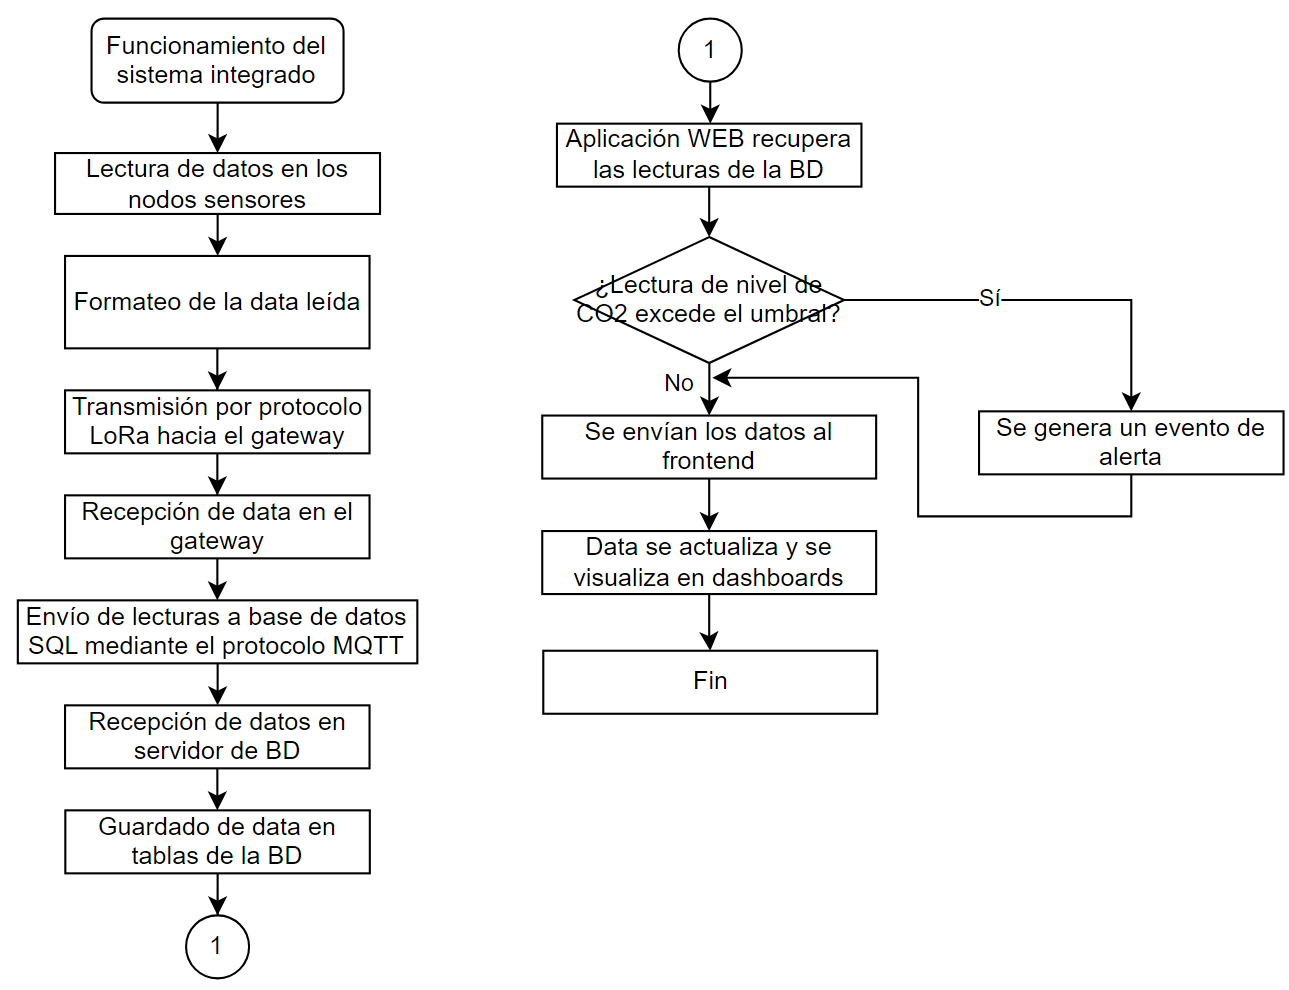
\includegraphics[width=\linewidth]{images/capitulo3/DF_integracion.png}
    \caption{Diagrama de flujo del funcionamiento del sistema}
    \label{fig:DF_integracion}
\end{figure}
